%%%%%%%%%%%%%%%%%%%%%%%%%% author.tex %%%%%%%%%%%%%%%%%%%%%%%%%
%
% sample root file for your contribution to a "contributed book"
%
% "contributed book"
%
% Use this file as a template for your own input.
%
%%%%%%%%%%%%%%%%%%%%%%%% Springer-Verlag %%%%%%%%%%%%%%%%%%%%%%%%%%


% RECOMMENDED %%%%%%%%%%%%%%%%%%%%%%%%%%%%%%%%%%%%%%%%%%%%%%%%%%%
\documentclass{svmult}

% choose options for [] as required from the list
% in the Reference Guide, Sect. 2.2

\usepackage{amssymb}         % assumes amsmath package installed
\usepackage{amsmath}         % assumes amsmath package installed
\usepackage{makeidx}         % allows index generation
\usepackage{graphicx}        % standard LaTeX graphics tool
                             % when including figure files
\usepackage{multicol}        % used for the two-column index
\usepackage[bottom]{footmisc}% places footnotes at page bottom
% etc.
% see the list of further useful packages
% in the Reference Guide, Sects. 2.3, 3.1-3.3

\makeindex             % used for the subject index
                       % please use the style sprmidx.sty with
                       % your makeindex program

\newcommand{\q}{\mathbf q}
\newcommand{\dq}{\dot {\mathbf q}}
\newcommand{\x}{\mathbf {x}}
\newcommand{\dx}{\dot {\mathbf x}}
\newcommand{\ProofBegin}{{\em Proof.} }
\newcommand{\ProofEnd}{\hfill $\diamondsuit$\\}

\newtheorem{fact}[theorem]{Proposition}
%%%%%%%%%%%%%%%%%%%%%%%%%%%%%%%%%%%%%%%%%%%%%%%%%%%%%%%%%%%%%%%%%%%%%

\begin{document}

\title{Exploiting Motor Modules in Modular Contexts}
% Use \titlerunning{Short Title} for an abbreviated version of
% your contribution title if the original one is too long
\author{Francesco Nori\inst{1}\and
Giorgio Metta\inst{1,2} \and Giulio Sandini\inst{1}}
% Use \authorrunning{Short Title} for an abbreviated version of
% your contribution title if the original one is too long
\institute{Italian Institute of Technology, via Morego 30,
16163 Genova
\texttt{francesco.nori@iit.it, giorgio.metta@iit.it, giulio.sandini@iit.it}
\and University of Genoa, Department of Communication 
Computer and System Sciences, Viale F. Causa 13,  16145
Genoa, Italy}
%
% Use the package "url.sty" to avoid
% problems with special characters
% used in your e-mail or web address
%
\maketitle

\abstract{Recently there has been a growing interest in modeling
motor control systems with modular structures. Such control
structures have many interesting properties, which have been
described in recent studies. We here focus on some properties which
are related to the fact that specific set of contexts can themselves
be modeled modularly. Specifically, we show that the adaptation of a
modular control structure can be guided by the modularity of
contexts, by means of interpreting the current unexperienced context
as the combination of previously experienced contexts.}
%% \title, \author and \abstract MUST be specified before \maketitle.

\section{Introduction}

Humans exhibit a broad repertoire of motor capabilities which can be
performed in a wide range of different environments and situations.
From the point of view of control theory, the problem of dealing
with different environmental situations is nontrivial and requires
significant adaptive capabilities. Even the simple movement of
lifting up an object, depends on many variables, both {\em internal
and external} to the body.
Examples of internal variables
are the state of the arm (i.e. joint angles and angular velocities)
and its dynamic parameters (i.e. masses , moments of inertia, etc.).
However, when interacting with the environment, motor commands need
to be adapted also to some {\em external variables} such as the
geometrical and dynamical parameters of lifted objects.
All these variables define what is generally called the context of
the movement. As the context of the movement alters the input-output
relationship of the controlled system, the motor command must be
tailored so as to take into account the current context. In everyday
life, humans interact with multiple different environments and their
possible combinations. Therefore, a fundamental question in motor
control concerns how the control system adapts to a continuously
changing operating context.

The adaptation of the motor control system to a continuously 
changing environment is a complex task. Noticeably, the dimensionality
of the context space grows exponentially with the number 
of alternatives/variables used to describe the context itself.
Therefore, this {\em curse of dimensionality} rules out any 
brute force approach for solving the context adaptation problem.
Moreover, recent studies have shown that nature have 
found much more interesting solutions. Specifically, in the 
following section we propose some experiments proposing the idea 
that the adaptation to new contexts can be achieved by means of 
linearly combining the knowledge about previously experienced contexts.

\subsection{Experimental evidence on modular organization of the motor control system}
\label{Sec:ExpEvid}

Recently, a huge amount of literature have shown that 
biological motor control systems are based on a continuous
adaptation of internal models. These models can be seen as
an internal representations used by the central nervous system
to handle the current context. Within this framework, there has been recently a major interest 
in modeling these internal models by means of combinations of a finite 
number of elementary modules. According to this modular architecture, 
multiple controllers co-exist, with each controller suitable for a 
specific context. If no controller is available for a given 
context, the individual controllers can be combined to generate 
an appropriate motor command. Therefore, even if internal models could be
learned by a single module, there seems to be at least three main
advantages \cite{WolpertKawato1998} related to their organization 
in multiple modules:

\begin{itemize}

\item \textbf{Modularity of contexts.} The contexts within which the model operates
can be themselves modular. Experiences of past contexts and objects
can be meaningfully combined; new situations can be often understood
in terms of combinations of previously experienced contexts.

\item \textbf{Modularity of motor learning.} In a modular structure only a subset
of the individual modules cooperate in a specific context.
Consequently, only these modules have a part in motor learning,
without affecting the motor behaviors already learned by other
modules. This situation seems more realistic than a global structure
where a unique module is capable of handling all possible contexts.
Within such a global framework, motor learning in a new context
possibly affects motor behaviors in other (previously experienced)
contexts.

\item \textbf{Dimensionality of generated motor acts.} By modulating 
the contribution of each module, a huge amount of new behaviors can 
be generated. In particular, the modules can be seen as a vocabulary 
of motor primitives, which are the building blocks for constructing 
complex novel motor acts.
 
\end{itemize}

Remarkably, there is experimental evidence supporting the hypothesis
that biological motor control systems are organized in modules. In
particular, Mussa-Ivaldi and Bizzi \cite{BizziMussa-Ivaldi} have shown
that this modularity is already present at the spinal cord level 
in the form of multiple goal directed muscle synergies acting at 
the level of individual limbs. Each synergy has been described 
in terms of the force field generated at the extremity of the limb.
Interestingly, the observed fields where limited in number (activated 
fields were grouped into few classes), goal
directed (the force field converged to toward an
equilibrium point) and  linearly combinable (the simultaneous 
stimulation led to vector summation of the generated forces). In our
opinion this experiment, though limited to frogs and rats, paves the 
way to interpret biological motor control systems (and the 
associated internal models) as modular structures. 


Concerning experiments with humans, there has been a growing interest
in understanding how internal models are organized in the central
nervous system. Interestingly, the existence and the adaptability 
of kinematic \cite{flangan95trajectory} and dynamic internal models 
\cite{Shadmehr} have been extensively proved. Remarkably, these two 
representations have been proved to be weakly intertwined \cite{krakauer99independent},
thus revealing a first level of modularity. 

A second level of modularity 
is revealed when considering human capability of switching 
between previously learned internal models. In particular, 
although the time course of adaptation to a novel context can 
extend over hours, restoring the pre-perturbation behavior is 
often faster \cite{welch93alternating,brashers-krug96consolidation}
thus suggesting the restoration of the previously acquired module. 

At a third level there is also evidence suggesting that 
previously acquired modules can be combined to generalize
in a new context which can be interpreted as the combination
of previously experienced contexts. In particular, in a 
kinematic scenario, it has been shown that two different 
visuomotor mappings can be learned 
\cite{ghahramani97modular} and these maps can be interpolated
to create new ones. Similarly, in a dynamic scenario, 
human subjects have shown the ability of combining previously 
acquired internal models when new contexts which can be
interpreted as the combination of previously acquired contexts.
Specifically, after learning the correct grasping forces 
for lifting two different objects, subjects have displayed
the ability of producing the correct force for lifting both
objects simultaneously without any training \cite{davidson04internal}.

As a concluding remark, the robustness displayed by biological motor control
systems seems to be the result of an extraordinary capability of adapting to
continuously changing contexts. This adaptation seems to be achieved in a twofold
manner: by a continuous update of existing modules and by the combination (switching)
of (between) previously learned modules. Remarkably, experiments suggest that the two
processes take advantage of different information: while adaptation 
can be attributed to performance errors \cite{Shadmehr}, switching and 
combination depend on sensory components of the context \cite{Shelhamer}. 

\subsection{Adaptive and modular motor control strategies}

Based on these findings, there has been recently a growing interest
in investigating the potentialities of \emph{adaptive and modular}
control schemes (refer to \cite{WolpertKawato1998, Mussa-Ivaldi}).
Within these investigations, the modular structure is often
formalized in terms of multiple forward/inverse models\footnote{Here an
forward model is considered to be a map from motor commands to the 
corresponding movement. Viceversa an inverse model corresponds to 
a map from desired movement to motor commands.}. Motor commands are 
usually obtained by combining these elementary internal models: different
combinations serve different contexts. Therefore, supposing that a set 
of possible operational contexts has been defined, two fundamental questions 
must be faced:

\begin{enumerate}

\item Is there a way to choose the elementary internal models so as to
cover all the contexts within a the specified set?

\item Given a set of internal models which appropriately cover the set
of contexts, how is the correct subset of internal models selected 
for the particular current context?

\end{enumerate}

Both questions have been already investigated in
\cite{WolpertKawato1998} and in \cite{MussaIvaldi1992BiolCyb} within
the function approximation framework. Recently, the same two
questions have been considered by \cite{NoriBiolCyb2005} within a
control theoretical framework. So far this novel approach has
been proved to provide new interesting results in answering the
first question (see \cite{NoriFrezzaCdc04} and
\cite{NoriPhDThesis}). In this work, we proceed along the
same line to answer the second question. Remarkably, (see Section
\ref{Sec:ExpEvid}) human behavioral studies have already shown 
that the module adaptation and selection processes rely mainly 
on performance errors and context related sensory information. 
Having in mind an application in the humanoid robotic field, we propose a
strategy to adaptively select a given set of inverse models. The
selection process is based both on the minimization of performance
errors and on context related sensory information. The key
features of the proposed control scheme are the following:

\begin{itemize}

\item \textbf{Minimum number of modules.} Previous works \cite{NoriPhDThesis}
have established the minimum number of modules which are necessary
to cover all the contexts in a specified set. The present paper will
describe how this minimality result can be fitted in the adaptive
selection of the modules.

\item \textbf{Linear combination of modules.} The theory of adaptive
control has been widely studied since the early seventies.
Interesting results have been obtained, especially in those
situations where some linearity properties can be proven and
exploited. In our case, linearity will be a property of the
considered set of admissible contexts.
\end{itemize}

The remaining sections are organized as follows. Section
\ref{Sec:SimpleReach} gives our formal definition of 
modular motor control strategy; a simple example is
analyzed and a solution is given.

\section{Reaching with a modular control structure} \label{Sec:SimpleReach}

In this section we give a formal definition of the motor
control modules. In a mathematical framework, the system
to be controlled will be described by the following differential 
equation:
\begin{eqnarray} \label{Eq:NonLinMod}
\mathbf {\dot x} = f (\mathbf x) + g(\mathbf x) \mathbf u
\end{eqnarray}
where $\mathbf x \in \mathbb R^n$ is the system state and 
the vector $\mathbf u  \in \mathbb R^m$ is the system input,
corresponding to our control variable. Different definitions
of modular control strategies can be given; here we follow the 
formalization which was originally proposed in \cite{BizziMussa-Ivaldi}
as a mathematical description of the experimentally observed
spinal force fields. Practically speaking the original control
variable $\mathbf u$ is replaced by the linear superposition
of a finite number of elementary control strategies 
$\{ \Phi^1(\mathbf x), \Phi^2(\mathbf x), \dots, \Phi^K(\mathbf x)\}$. Therefore we have:
\begin{eqnarray} \label{Eq:BasicModelControl}
\mathbf u = \sum_{k=1}^K \lambda_k \Phi^k(\mathbf x),
\end{eqnarray}
where the new control variables are the mixing coefficients 
$\lambda_1, \lambda_2, \dots, \lambda_K$ which are assumed to be 
constant during the execution of a single movement. 

To exemplify the proposed ideas we will consider a specific task, 
nominally reaching. Within this framework, the system to be controlled
will be a mathematical model of the limb dynamics, which can always
be written as follows:
\begin{eqnarray} \label{Eq:KinChainModel}
M(\mathbf{q}) \ddot{\mathbf{q}} +
C(\mathbf{q},\dot{\mathbf{q}})\dot{\mathbf{q}} + g(\mathbf{q}) =
\mathbf{u},
\end{eqnarray}
where $\mathbf{q}$ are the generalized coordinates which describe
the pose of the kinematic chain, $\mathbf{u}$ are the control
variables (nominally the forces applied at the joints) and the
quantities $M$, $C$ and  $g$ are the inertia, Coriolis and
gravitational components. Remarkably, \eqref{Eq:KinChainModel}
can always be written in the state space form 
\eqref{Eq:BasicModelControl} defining $\mathbf x = [\mathbf q, 
\dot{\mathbf q}]$.
 
The problem of reaching consists in finding an input that drives the
system configuration $\mathbf x$ to any desired reachable state $\mathbf x_f$. If
our control input were the original (time variant) input variable $\mathbf u$, then
the problem would be easily solved by using classical control techniques
\cite{MurrayLeeSastry}. In the modular structure framework, the input
variables are the (time invariant) combinators and therefore a major attention 
should be posed in selecting the modules. If we do not choose the functions
$\Phi_k$ properly, some configurations (reachable by a suitable
choice of the original input $\mathbf u$) might be no longer reachable 
by the new input variables. Formally speaking, the system 
\eqref{Eq:KinChainModel} might lost its controllability by imposing
the modular structure \eqref{Eq:BasicModelControl} on its input.
As to this concern, the following problem has been formulated:

\begin{problem}[Synthesis of Elementary Controls for Reaching] \label{Prb:ElemContrSynth}
Find a set of modules $\{\Phi^1$, $\dots$,
$\Phi^K\}$ and a continuously differentiable function
$\lambda(\cdot)$, such that for every desired reachable state 
$\mathbf x_f$ the input:
\begin{eqnarray} \label{Eq:CombinedInput}
\mathbf u = \sum_{k=1}^K \lambda_k(\mathbf x_f) \Phi^k(\mathbf x)
\end{eqnarray}
steers the system (\ref{Eq:KinChainModel}) to the state $\mathbf x_f$.
\end{problem}

As it was previously pointed out, previous attempts to solve 
the above controllability problem were based on a function 
approximation framework \cite{WolpertKawato1998,MussaIvaldi1992BiolCyb}.
The main drawback of this approach is the high number of required modules.
Such a drawback follows from a quite general principle: without any a priori knowledge on
the function to be approximated, the more the modules are the better 
the approximation will be. Here we follow a different solution 
originally proposed in \cite{NoriFrezzaNolcos04} and based on the
idea of maintaining the number of primitives as low as possible.
Remarkably, the proposed solution is composed by $n+1$ primitives\footnote{
Remember that $n$ is the state space dimensionality, i.e. $\x \in \mathbb R^n$.}
which is proved to be the minimum number under suitable hypotheses 
(see Section \ref{Sec:MinNumPrimitives}). Details on how to 
construct such a minimal solution to Prb. \ref{Prb:ElemContrSynth}
can be found in \cite{NoriBiolCyb2005}.

\section{Reaching in different contexts}

In order to immerse the reaching action into different contexts,
we now consider the same movement while holding objects with
different masses and inertias. Within this framework, a successful
execution of the reaching movements requires a control action which
should adapt to the current context. Since the controlled
system\footnote{Within this framework the controlled system is
composed of the arm {\em and} the held object.} changes its properties 
with the context, suitable changes should be imposed on the control action.
It is important to notice that the considered set of contexts is itself
modular. In particular, two different objects can be held simultaneously 
thus producing a situation which is exactly the combination of the two 
contexts corresponding to holding separately the two objects.

Once again the dynamical system to be controlled can be expressed as
a differential equation with the structure of \eqref{Eq:KinChainModel}.
However in this case the matrices $M$, $C$ and $g$ depend on the 
context as consequence of the fact that the limb dynamical 
parameters change when holding different objects. To model this 
situation we explicitly take into account that the limb dynamical parameters, grouped in 
a vector $\mathbf p$, vary with the context. Specifically, if we 
consider that the objects can be attached to any of the limb links,
we have:
\begin{eqnarray}
\mathbf p = \begin{bmatrix} m_i & I^i_1 & \dots & I^i_6  & c^i_x & c^i_y & c^i_z
\end{bmatrix}^\top_{i = 1 \dots n},
\end{eqnarray}
where $m_i$ is the mass of the $i^{th}$ link, $I^i_1$, $\dots$,
$I^i_6$ represent the entries of the symmetric inertia tensor, and
$\left[ c^i_x, c^i_y, c^i_z \right]^\top$ is the center of mass position.
The system to be controlled is therefore:
\begin{eqnarray} \label{Eq:KinChainModelContext}
M_{\mathbf p}(\mathbf{q}) \ddot{\mathbf{q}} + C_{\mathbf
p}(\mathbf{q},\dot{\mathbf{q}})\dot{\mathbf{q}} + g_{\mathbf
p}(\mathbf{q}) = \mathbf{u},
\end{eqnarray}
where we explicitly indicate that the controlled dynamical system
depends on the contexts which have been parameterized with 
the vector $\mathbf p$. Remarkably, the proposed set of contexts 
is itself modular. It can indeed be proved that \eqref{Eq:KinChainModelContext}
can be rewritten as (see \cite{Kozlowski}):
\begin{eqnarray} \label{Eq:ContextModularity}
\sum_{j=1}^J \Psi_j(\mathbf p) Y^j(\mathbf q, \dot{\mathbf q},
\ddot{\mathbf q}) = \mathbf u.
\end{eqnarray}
This is a crucial property which is fundamental to prove the results
which will be claimed in the rest of this paper.


\section{Modular control action}

In this section we formalize our concept of modular control action.
The proposed formalization is biologically inspired and has been
originally proposed by \cite{BizziMussa-Ivaldi}. Specifically,
experiments on frogs and rats have shown that their motor systems is
organized into a {\em finite number of modules}.  Each module has
been described in terms of the muscular synergy evoked by the
microstimulation of specific interneurons in the spinal cord. These
modules can be {\em linearly combined} to achieve a wide repertoire
of different movements. A mathematical model of these findings has
been proposed again by \cite{BizziMussa-Ivaldi}:
\begin{eqnarray} \label{Eq:BasicModelControlv2}
\mathbf u = \sum_{k=1}^K \lambda_k \Phi^k(\mathbf q, \dot{\mathbf
q}).
\end{eqnarray}
Practically, the system (\ref{Eq:KinChainModel}) is controlled by
means of a linear combination of a finite number of modules
$\Phi^k(\mathbf q, \dot{\mathbf q})$, which can be seen as
elementary control actions. The control signals are no longer the
forces $\mathbf u$ but the vector $\left[ \lambda_1, \dots,
\lambda_K \right]^\top = \lambda$ used to combine the modules.

\subsubsection{Modules for handling admissible contexts} \label{Sec:ModContexts}

In this paper, we consider the problem of solving problem 1 in
different contexts. Practically, we face the following problem where
instead of controlling (\ref{Eq:KinChainModel}) we want to control
(\ref{Eq:KinChainModelContext}) which is context dependent.
\\
\\
\textbf{Problem 2:} {\em find a set of modules $\{\Phi^1$, $\dots$,
$\Phi^K\}$ and a continuously differentiable function
$\lambda(\cdot, \cdot)$, such that for every desired final state
$\mathbf q_f$ and for every possible context $\mathbf p$ the input:
\begin{eqnarray}
\mathbf u = \sum_{k=1}^K \lambda_k(\mathbf q_f, \mathbf p)
\Phi^k(\mathbf q, \dot{\mathbf q})
\end{eqnarray}
steers the system (\ref{Eq:KinChainModelContext}) to the configuration $\mathbf q_f$.}\\
\\
Obviously the proposed problem is related to the question posed in
the introduction: is there a way to choose the elementary (inverse)
models so as to cover all the contexts within a specified set? The
answer turns out to be `yes'. Specifically, a complete procedure for
constructing a solution of problem 2 has been proposed in
\cite{NoriPhDThesis}. The solution turns out to have the following
structure:
\begin{eqnarray} \label{Eq:BasicModelControlContext}
\mathbf u = \sum_{i = 1}^I \sum_{j = 1}^J \lambda_i(\mathbf q_f)
\mu_j(\mathbf p) \Phi^{i,j}(\mathbf q, \dot{\mathbf q}),
\end{eqnarray}
where $\{\Phi^{1,j}$, $\dots$, $\Phi^{I,j}\}$ is a solution to
problem 1 for a specific context $\mathbf p^j$.

\subsection{Adaptive modules combination}

In the present section we consider the problem of adaptively
combining a given set of modules. The first part of the section,
describes a method for adaptively adjusting the modules selection on
the basis of performance errors. In the second part, we suggest how
adaptation can be made on the basis of context related information.

\subsection{Performance error based adaptation}
\label{Sec:ErrorBasedAdapt}

In many situations, the context of the movement is not known {\em a
priori}. Within our formulation, if the context $\mathbf p$ is
unknown, we cannot compute the way the modules have to be combined.
This is a consequence of the fact that the way modules are combined
depends not only on the desired final position $\mathbf q_f$ but
also on the current context $\mathbf p$. A possible solution
consists in adaptively choosing $\mu_j$ (which are context
dependent) on the basis of available data. When the only information
available is the performance error\footnote{The performance error
$\mathbf s$ measures the difference between the desired reaching
trajectory $\mathbf q^d$ and the actual trajectory $\q$. Further
details can be found in \cite{Kozlowski}}, we can reformulate the
estimation problem in terms of an adaptive control problem. It can
be proven that a way to successfully reach the desired final
position $\mathbf q_f$ consists in adaptively adjusting $\mu_j$
according to the following differential law:
\begin{eqnarray} \label{Eq:UpdateCombin}
\frac{d}{dt}{\mu_j} = - \mathbf s^\top \left[ \sum_{i = 1}^I
\lambda_i(\mathbf q_f) \Phi^{i,j}(\mathbf q, \dot{\mathbf q})
\right],
\end{eqnarray}
where $\mathbf s$ is the performance error (see \cite{Kozlowski} for
details). A mathematical proof of the system stability properties is
out of the scope of the present paper and is therefore omitted. It
suffices to say that, in fact, it can be proven that
(\ref{Eq:UpdateCombin}) leads to a stable system.

\subsection{Context based adaptation}

Humans exhibit an extraordinary capability of exploiting previous
experiences in a nontrivial way. Consider for example the problem of
lifting up an object. Clearly, the movement is preplanned on the
basis of some {\em a priori} information\footnote{A very common
situation reveals that movements are preplanned on the basis of some
a priori information. Consider for example the movement of lifting
up an empty bottle. Sometimes we misinterpret the context,
considering the bottle full and therefore using a wrong a priori
information. In these situations, the resulting movement presents an
overshoot, thus revealing that a wrong a priori information has been
used.}. How can we create this a priori information when lifting an
object that we have never lifted before?

Clearly, we can obtain a priori information of unknown objects on
the basis of similarity. If an unknown object is similar to a known
one, then the same a priori information can be used. We here show
that another way to retrieve a priori information consists in
interpreting an unknown object as the combination of two or more
known objects.

Consider again our dynamic model of the arm holding an object:
\begin{eqnarray}
M_{\mathbf p}(\mathbf{q}) \ddot{\mathbf{q}} + C_{\mathbf
p}(\mathbf{q},\dot{\mathbf{q}})\dot{\mathbf{q}} + g_{\mathbf
p}(\mathbf{q}) = \mathbf u,
\end{eqnarray}
which can be rewritten as:
\begin{eqnarray} \label{Eq:DynMod}
Y_{\mathbf p}(\mathbf q, \dot{\mathbf q}, \ddot{\mathbf q}) =
\mathbf u.
\end{eqnarray}
Each context is described by a specific vector $\mathbf p$. Let
$\mathbf p^{\mathcal A}$ indicate the context of the arm (denoted
here with the letter $\mathcal A$) not holding any object. Let
$\mathbf p^{\mathcal A \cup \mathcal O}$ indicate the arm holding
the object $\mathcal O$. Observe that the notation helps in keeping
in mind that this second context corresponds to moving the arm {\em
and} the object. Consider now two different objects and assume that
these two objects are known, in the sense that we already know how
they affect the dynamics of our arm\footnote{It is well known that
our sensory motor system is capable of learning how external objects
affect the dynamics of its limbs. As a matter of fact, see
\cite{Shadmehr}.}. Can we make any a priori assumption on how
holding two objects simultaneously will affect the dynamics of the
arm? Said in other terms, can we make an hypothesis on $Y_{\mathbf
p}$ when holding the two objects?

The answer to the question above is `yes'. Consider a situation in
which the arm is first moved without holding any object. In this
first stage the dynamics of the arm can be learnt. Let these
dynamics be:
\begin{eqnarray} \label{Eq:DynModArmAlone}
Y_{\mathbf p^{\mathcal A}}(\mathbf q, \dot{\mathbf q}, \ddot{\mathbf
q}) = \mathbf u.
\end{eqnarray}
In a second stage, the dynamics of the arm holding the object are
learnt. Let these dynamics be:
\begin{eqnarray} \label{Eq:DynModArmObject}
Y_{\mathbf p^{\mathcal A \cup \mathcal O_1}}(\mathbf q, \dot{\mathbf
q}, \ddot{\mathbf q}) = \mathbf u.
\end{eqnarray}
Obviously, we cannot learn the dynamics of the object alone since
the only way to interact with the object consists in holding it with
the arm, which has its own dynamics. However, we can associate to
the object $\mathcal O_1$ the dynamics $Y_{\mathbf p^{\mathcal
O_1}}$ obtained as the difference between the dynamics with and
without the object, i.e.:
\begin{multline} \label{Eq:DynModArmObjectDiff}
Y_{\mathbf p^{\mathcal O_1}}(\mathbf q, \dot{\mathbf q},
\ddot{\mathbf q}) = \\ Y_{\mathbf p^{\mathcal A \cup \mathcal
O_1}}(\mathbf q, \dot{\mathbf q}, \ddot{\mathbf q}) - Y_{\mathbf
p^{\mathcal A}}(\mathbf q, \dot{\mathbf q}, \ddot{\mathbf q}).
\end{multline}
In a third stage the dynamics of the arm holding a second object
$\mathcal O_2$ are learnt. Also in this case the quantity
$Y_{\mathbf p^{\mathcal O_2}} = Y_{\mathbf p^{\mathcal A, \mathcal
O_2}} - Y_{\mathbf p^{\mathcal A}}$ is associated with the object.
At this stage, we have learnt the dynamics $Y_{\mathbf p^{\mathcal
A}}$ of the arm, and the dynamics $Y_{\mathbf p^{\mathcal O_1}}$,
$Y_{\mathbf p^{\mathcal O_2}}$ associated with the two objects
${\mathcal O_1}$ and ${\mathcal O_2}$. Let's now create a new object
$\mathcal O_s$ composing the two known objects. Using once more the
notation above, we can say $\mathcal O_s = \mathcal O_1 \cup
\mathcal O_2$. What can we conclude about $Y_{\mathbf p^{\mathcal A
\cup \mathcal O_s}} = Y_{\mathbf p^{\mathcal A \cup \mathcal O_1
\cup \mathcal O_2 }}$, i.e. about the dynamics of the arm holding
the two objects simultaneously? Interestingly, it can be shown that:
\begin{eqnarray} \label{Eq:AdditivityContexts}
Y_{\mathbf p^{\mathcal A \cup \mathcal O_1 \cup \mathcal O_2}} =
Y_{\mathbf p^{\mathcal A}} + Y_{\mathbf p^{\mathcal O_1}} +
Y_{\mathbf p^{\mathcal O_2}}.
\end{eqnarray}
Practically, the combination of contexts corresponds to the
additivity of the corresponding dynamics. Using this property, it
can be shown that an equation similar to
(\ref{Eq:AdditivityContexts}) holds for the context dependent
coefficients in (\ref{Eq:BasicModelControlContext}). In particular,
we have that the coefficients $\mu_j(\mathbf p)$ satisfy the
following:
\begin{multline} \label{Eq:AdditivityCoeff}
\mu_j({\mathbf p^{\mathcal A \cup \mathcal O_1 \cup \mathcal O_2}})
= \\ \mu_j({\mathbf p^{\mathcal A}}) + \mu_j({\mathbf p^{\mathcal
O_1}}) + \mu_j({\mathbf p^{\mathcal O_2}}),
\end{multline}
where, once more, the quantities $\mu_j({\mathbf p^{\mathcal O_1}})$
and $\mu_j({\mathbf p^{\mathcal O_2}})$ are defined as the
difference of $\mu_j$ with and without the object, i.e.:
\begin{subequations}\label{Eq:AdditivityCoeffObj}
\begin{eqnarray}
\mu_j({\mathbf p^{\mathcal O_1}}) & = & \mu_j({\mathbf p^{\mathcal A
\cup \mathcal O_1}}) - \mu_j({\mathbf p^{\mathcal A}}), \\
\mu_j({\mathbf p^{\mathcal O_2}}) & = & \mu_j({\mathbf p^{\mathcal A
\cup \mathcal O_2}}) - \mu_j({\mathbf p^{\mathcal A}}).
\end{eqnarray}
\end{subequations}
Therefore, consider an unexperienced context (${\mathbf p^{\mathcal
A \cup \mathcal O_1 \cup \mathcal O_2}}$) which can be interpreted
as the combination of previously experienced contexts (${\mathbf
p^{\mathcal A }}$, ${\mathbf p^{\mathcal A \cup \mathcal O_1}}$,
${\mathbf p^{\mathcal A \cup \mathcal O_2}}$). Then, equations
(\ref{Eq:AdditivityCoeff}) and (\ref{Eq:AdditivityCoeffObj}) give a
way to combine the modules in order to handle the current
unexperienced context. Clearly, this procedure needs to be combined
with the performance error based adaptation (proposed in Section
\ref{Sec:ErrorBasedAdapt}) in order to learn the combination of
modules in contexts which cannot be interpreted as the combination
of known contexts.

\section{Future works}

In the framework of motor control, this paper proposes a method for
performing on-line learning of reaching movements. The proposed
control structure is biologically compatible and is proven to be
very useful when dealing with modular contexts. A crucial step in
our future work will be the implementation of the system in a
humanoid robot. The idea is to use sensors (mainly vision) to
extract context related information and interpret the current
context as the combination of previously experienced contexts. As
previously explained, this information can be used to adapt a given
set of modules to the current context. In our personal opinion, the
proposed architecture is potentially efficient in dealing with
multiple and modular contexts determined, for instance, by
manipulating/holding different objects.

\section{Conclusions}

Modular control structures are appealing since there exist contexts
which can be modular as well. In the present paper we have
considered a simple movement (moving the arm towards a target)
within different contexts (handling different objects). Intuitively,
a modular control structure is best suited to operate within modular
contexts. In the specific problem of moving the arm while holding
different objects, we have shown that the system dynamics are
modular themselves. Taking advantage of this property we have shown
that a modular control structure is capable of handling multiple
contexts. Finally, two ways to adaptively combine the modules has
been proposed. A first adaptation is based on performance errors
only. A second adaptation, which relies on the first, is used to
combine the modules in unexperienced contexts which can be
interpreted as the combination of previously experienced contexts.

\section*{Acknowledgements}

The work presented in this paper has been supported by the project
\textsc{Robot Cub} (IST-2004-004370) and by the project
\textsc{Neurobotics} (IST-2003-511492). Both projects are funded by
the European Union through the Sixth Framework Programme for
Research and Technological Development (FP6).

\appendix

\section{Minimum Number of Motion Primitives} \label{Sec:MinNumPrimitives}

\subsection{Lower Bound on the Number of Elementary Controls} \label{Sec:LowerBound}

In this Section we prove that any given solution of Prb.
\ref{Prb:ElemContrSynth} is composed by at least $n$
elementary controls, i.e. $K \geq n$. Before giving the main
result, we prove the following lemma, claiming the injectivity of
the function $\lambda$. In the following the set of reachable states
is denoted $\mathcal X \subseteq \mathbb R^n$.

\begin{lemma} \label{Lem:OneToOne}
Let $\{\Phi^1$, $\dots$, $\Phi^K\}$ and $\lambda : \mathcal X
\rightarrow \mathbb R^K$ be a solution to
Problem \ref{Prb:ElemContrSynth}. Then $\lambda(\x_f)$ is injective.
\end{lemma}

\ProofBegin Suppose by contradiction that there exist 
$\mathbf x_f^1$ and $\mathbf x_f^2$ such
that $\mathbf x_f^1 \neq \mathbf x_f^2$ but $\lambda(\mathbf
x_f^1) = \lambda(\mathbf x_f^2)$. Define:
\begin{eqnarray}
\mathbf u^1 & \triangleq & \sum_{k=1}^K \lambda_k(\mathbf
x_f^1) \Phi^k(\mathbf x), \\ \mathbf u^2 & \triangleq &
\sum_{k=1}^K \lambda_k(\mathbf x_f^2) \Phi^k(\mathbf x).
\end{eqnarray}
Under the given assumption $\mathbf u^1 = \mathbf u^2$, but this
contradicts the fact that $\mathbf u^1$ drives the system to 
$\mathbf x_f^1 \neq \mathbf x_f^2$. By contradiction, this proves 
that $\lambda$ is injective. \ProofEnd

\begin{fact} \label{Pro:LowerBound}
Let $\{\Phi^1$, $\dots$, $\Phi^K\}$ and $\lambda : \mathcal X
\rightarrow \mathbb R^K$ be a solution to Problem
\ref{Prb:ElemContrSynth}. Then $K \geq n$.
\end{fact}

\ProofBegin Using Lemma \ref{Lem:OneToOne}, we have that
$\lambda(\cdot)$ is a continuously differentiable injective
function from an open subset of $\mathbb R^n$ to $\mathbb R^K$. It
can be proved that this implies $K \geq n$ (see \cite{Boothby} for 
details). \ProofEnd
%%%%%%%%%%%%%%%%%%%%%%%%%%%%%%%%%%%%%%%%%%%%%%%%%%%%%%%%%%%%%%%%%%%%%%%%%%


%%%%%%%%%%%%%%%%%%%%%%%%%%%%%%%%%%%%%%%%%%%%%%%%%%%%%%%%%%%%%%%%%%%%%%%%%%

\subsection{Minimum number of elementary controls} \label{Sec:MinNumPrimitivesNonLin}

We have shown that we need at least $n$ 
primitives to preserve controllability. We here show that $n$ are not
sufficient under suitable assumptions. Let's consider an affine nonlinear system 
of type \eqref{Eq:NonLinMod}. Let $\{\Phi^1$, $\dots$, $\Phi^K\}$, $\lambda 
: \mathcal X \rightarrow \mathbb R^K$ be a solution to Problem 
\ref{Prb:ElemContrSynth}. Moreover, define $\mathcal
X_{\mbox{eq}} \subset \mathcal X$ to be the set of equilibrium
points with $\mathbf u = 0$, i.e. $\mathbf x_f \in \mathcal
X_{\mbox{eq}}$ if and only if $f(\mathbf x_f) = 0$. The proof of
the main result requires the following additional assumption.
\\
\\
\textbf{(HP)}. $\mathcal X_{\mbox{eq}} \neq \emptyset$ and
$\forall \x_f \in \mathcal X_{\mbox{eq}}$ the solution of the
following differential equation:
\begin{eqnarray}
\left\{ \begin{array} {l} \mathbf {\dot x} = f (\mathbf x) +
g(\mathbf x) \sum_{k=1}^K \lambda_k(\x_f) \Phi^k(\x, t)\\
\mathbf x(0) = \x_f
\end{array} \right. .
\end{eqnarray}
is $\mathbf x(t) \equiv \mathbf x_f$, $\forall t \in [0, T]$.
Basically, this is equivalent to requiring that if we start at an
equilibrium point and we want to reach the same equilibrium point,
then this is accomplished leaving the system in the same position
for the entire time interval.

\begin{theorem} \label{Th:MinNumPrimNonLin}
Let $\{\Phi^1, \dots, \Phi^K\}$, $\lambda: \mathcal X \rightarrow
\mathbb R^K$ be a solution to Problem
\ref{Prb:ElemContrSynth} with dynamics given by
(\ref{Eq:NonLinMod}). Moreover, assume that for the
given solution, (HP) holds. Then $K \geq n+1$.
\end{theorem}

\ProofBegin Suppose by contradiction that $K < n + 1$. Since we
have shown that $K \geq n$ we have only one possibility left out:
$K=n$. Define:
\begin{eqnarray}
\varPhi(\x, t) \triangleq \begin{bmatrix} \Phi^1(\x, t) & \dots &
\Phi^n(\x, t) \end{bmatrix} \qquad \lambda(\x_f) \triangleq \begin{bmatrix} \lambda_1(\x_f) & \dots &
\lambda_n(\x_f) \end{bmatrix}^\top,
\end{eqnarray}
so that we have:
\begin{eqnarray}
\sum_{k=1}^n \lambda_k(\x_f) \Phi^k(\x, t) = \varPhi(\x, t)
\lambda(\x_f).
\end{eqnarray}
Since the proposed primitives solve Prb.
\ref{Prb:ElemContrSynth}, the following system:
\begin{eqnarray} \label{Eq:BasicSystemControlSimply}
\left\{ \begin{array} {l} \mathbf {\dot x} = f (\mathbf x) +
g(\mathbf x) \varPhi(\x, t) \lambda(\x_f) \\
\mathbf x(0) = \x_0 \in \mathcal X
\end{array} \right. ,
\end{eqnarray}
converges to $\mathbf x_f$, $\forall \x_f \in \mathcal X$
regardless of the initial condition. Consider $\x_f \in \mathcal
X_{\mbox{eq}}$ and $\mathbf x(0) = \x_f$. Using (HP) in
(\ref{Eq:BasicSystemControlSimply}), we get:
\begin{eqnarray} \label{Eq:IdentNullControlAct}
g(\mathbf x_f) \varPhi(\x_f, t) \lambda(\x_f) = 0, \quad \quad
\forall t \in [0, T].
\end{eqnarray}
Now, let's use the fact that the image of $\mathcal X$ under
$\lambda: \mathcal X \rightarrow \mathbb R^n$ is an open set in $\mathbb R^n$.
This is consequence of the fact that $\lambda$ is injective and
$\mathcal C^1(\mathcal X)$ with $\mathcal X$ open (see \cite{Boothby} for details). If
$\mbox{Im}_\lambda(\mathcal X)$ is open and $\lambda(\x_f) \in
\mbox{Im}_\lambda(\mathcal X)$, we can always find $\mu \neq 1$
such that $\mu \lambda(\x_f) \in \mbox{Im}_\lambda(\mathcal X)$;
we only need to take $|1-\mu|$ small enough. Therefore, there
always exists $\tilde \x_f \in \mathcal X$, such that
$\lambda(\tilde \x_f) = \mu \lambda(\x_f)$. According to the given
hypothesis, the following system:
\begin{eqnarray} \label{Eq:ControlledSysTilde}
\left\{ \begin{array} {l} \mathbf {\dot x} = f (\mathbf x) +
g(\mathbf x) \varPhi(\x, t) \lambda(\tilde \x_f) \\
\mathbf x(0) = \x_0 \in \mathcal X
\end{array} \right. ,
\end{eqnarray}
should converge to $\tilde \x_f$ regardless of the initial
condition. However, take $\mathbf x_0 = \x_f$, and observe that
the corresponding trajectory is given by $\x(t) \equiv \x_f$,
$\forall t \in [0, T]$ since we have:
\begin{eqnarray*}
\mathbf {\dot x} = f (\mathbf x_f) + g(\mathbf x_f) \varPhi(\x_f,
t) \lambda(\tilde \x_f) = \mu g(\mathbf x_f) \varPhi(\x_f, t)
\lambda(\x_f) \stackrel{
(\ref{Eq:IdentNullControlAct})}{=} 0 \quad \forall t \in
[0, T].
\end{eqnarray*}
Therefore, we have found an initial condition for
(\ref{Eq:ControlledSysTilde}) that is not driven to $\tilde
\x_f$. This is in contradiction with our hypothesis.\ProofEnd
%%%%%%%%%%%%%%%%%%%%%%%%%%%%%%%%%%%%%%%%%%%%%%%%%%%%%%%%%%%%%%%%%%%%%%%%%%

\section{Section Heading}
\label{sec:1}
% Always give a unique label
% and use \ref{<label>} for cross-references
% and \cite{<label>} for bibliographic references
% use \sectionmark{}
% to alter or adjust the section heading in the running head
Your text goes here. Use the \LaTeX\ automatism for your citations.

\subsection{Subsection Heading}
\label{sec:2}
Your text goes here.

\begin{equation}
\vec{a}\times\vec{b}=\vec{c}
\end{equation}

\subsubsection{Subsubsection Heading}
Your text goes here. Use the \LaTeX\ automatism for cross-references as
well as for your citations, see Sect.~\ref{sec:1}.

\paragraph{Paragraph Heading} %
Your text goes here.

\subparagraph{Subparagraph Heading.} Your text goes here.%
%
\index{paragraph}
% Use the \index{} command to code your index words
%
% For tables use
%
\begin{table}
\centering
\caption{Please write your table caption here}
\label{tab:1}       % Give a unique label
%
% For LaTeX tables use
%
\begin{tabular}{lll}
\hline\noalign{\smallskip}
first & second & third  \\
\noalign{\smallskip}\hline\noalign{\smallskip}
number & number & number \\
number & number & number \\
\noalign{\smallskip}\hline
\end{tabular}
\end{table}
%
%
% For figures use
%
\begin{figure}
\centering
% Use the relevant command for your figure-insertion program
% to insert the figure file.
% For example, with the option graphics use
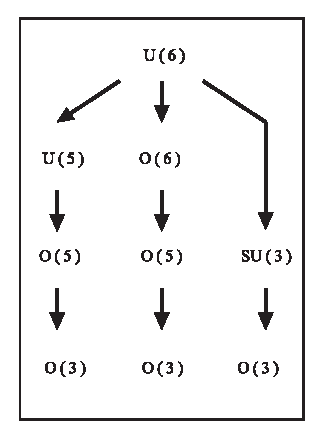
\includegraphics[height=4cm]{figure.eps}
%
% If not, use
%\picplace{5cm}{2cm} % Give the correct figure height and width in cm
%
\caption{Please write your figure caption here}
\label{fig:1}       % Give a unique label
\end{figure}
%
% For built-in environments use
%
\begin{theorem}
Theorem text\footnote{Footnote} goes here.
\end{theorem}
%
% or
%
\begin{lemma}
Lemma text goes here.
\end{lemma}
%
%
% BibTeX users please use
% \bibliographystyle{}
% \bibliography{}
%
% Non-BibTeX users please follow the syntax
% the syntax of "referenc.tex" for your own citations

\bibliographystyle{alpha}
\bibliography{author}


%%%%%%%%%%%%%%%%%%%%%%%%%%%%%%%%%%%%%%%%%%%%%%%%%%%%%%%%%%%%%%%%%%%%%%

%%%%%%%%%%%%%%%%%%%%%%%%%%%%%%%%%%%%%%%%%%%%%%%%%%%%%%%%%%%%%%%%%%%%%%

%\printindex
\end{document}
